%%%%%%%%%%%%%%%%%%%%%%%%%%%%%%%%%%%%%%%%%%%%%%%%%%%%%%%%%%%
%                       EXPOSITION DU SUJET               %
%%%%%%%%%%%%%%%%%%%%%%%%%%%%%%%%%%%%%%%%%%%%%%%%%%%%%%%%%%%

Le traitement d'images est un ensemble de méthodes permettant d'étudier et de transformer une ou plusieurs images à l'aide de moyens mathématiques et numériques. Le principe du traitement d'images consiste à extraire certaines informations de celles-ci, afin de les étudier ou de les modifier.Il est utilisé dans beaucoup d'applications telles que l'amélioration du contraste, l'application d'un filtre(flou, lissage, changement de couleurs), ou encore les détections et identifications d'objets par exemple. 

Dans ce rapport, nous nous intéresserons à l'incrustation d'images. À partir de deux images, comment sélectionner une partie de la première et l'incruster de la manière la plus naturelle possible dans la seconde ? 
\newline
Afin d'éclaircir nos propos et d'identifier les problèmes que nous devons résoudre, voici un exemple de ce que nous souhaitons faire.\newline
Nous disposons des deux images présentées ci-dessous, l'image T(arget) et l'image S(ource). 
\newline
\begin{figure}[!htb]
   \begin{minipage}{0.48\textwidth}
     \centering
     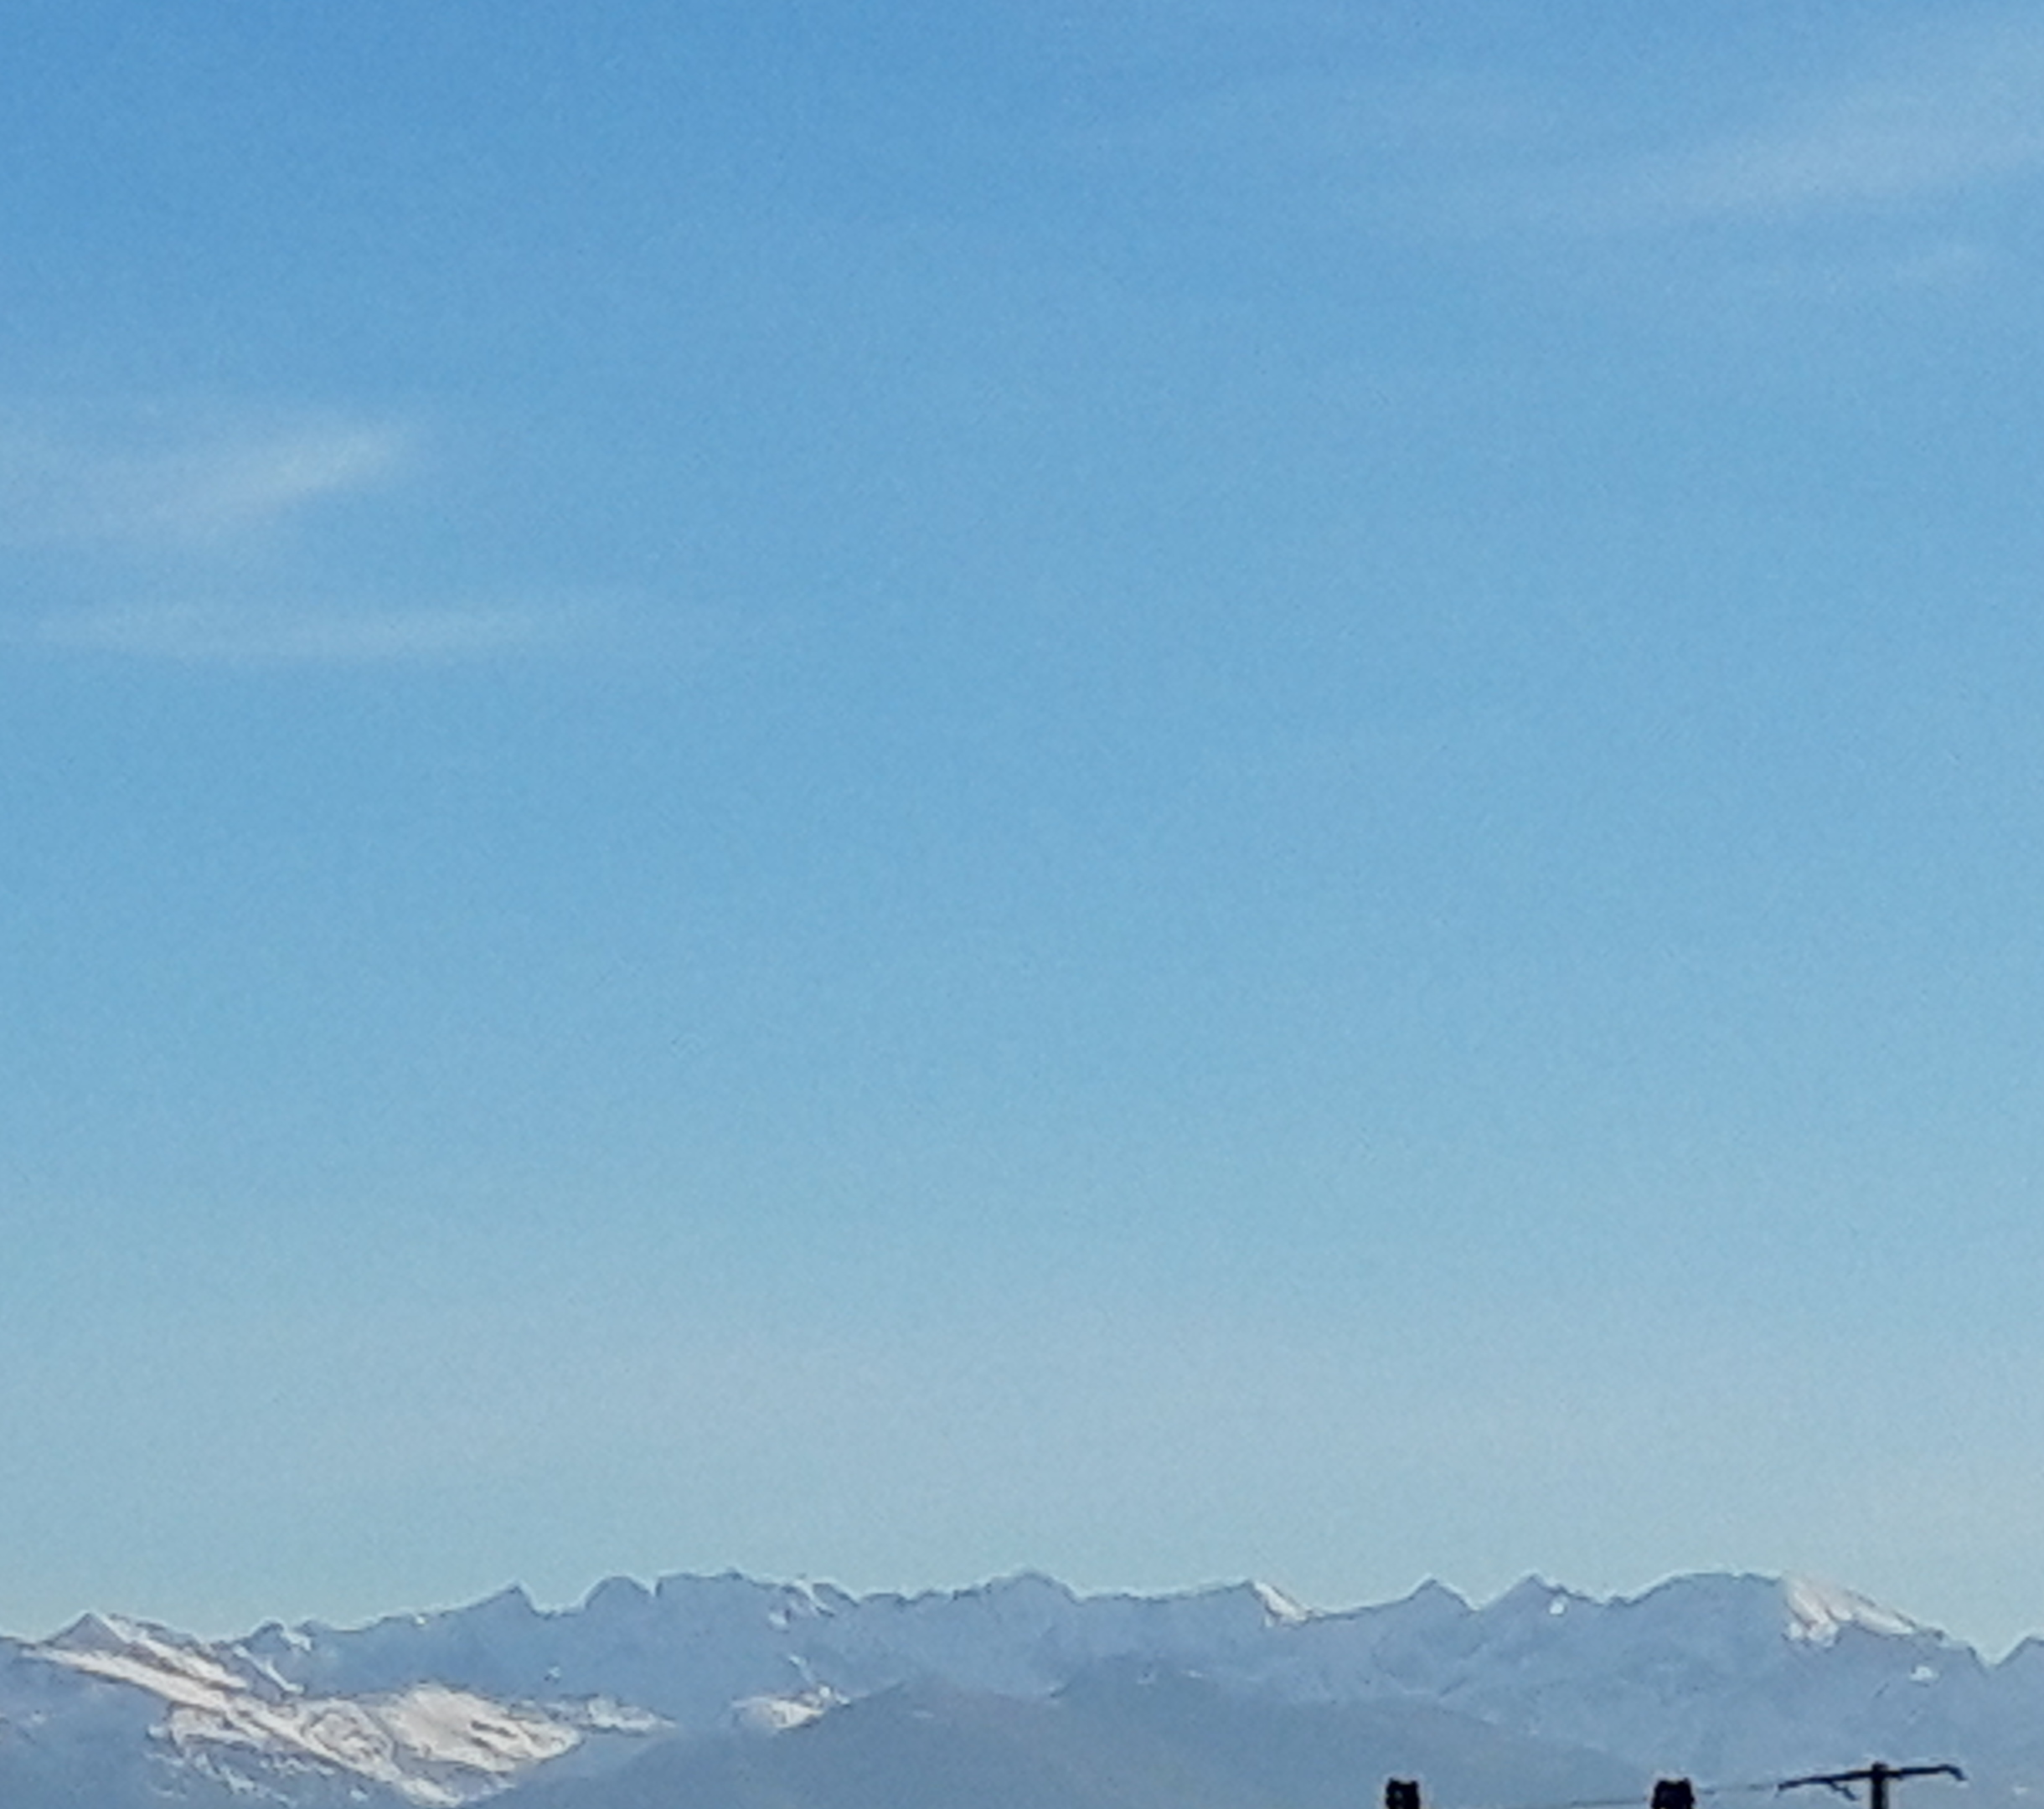
\includegraphics[width = 150pt]{Images/Montagne.jpg}
     \caption{Image T}
      \end{minipage}\hfill
   \begin{minipage}{0.48\textwidth}
     \centering
     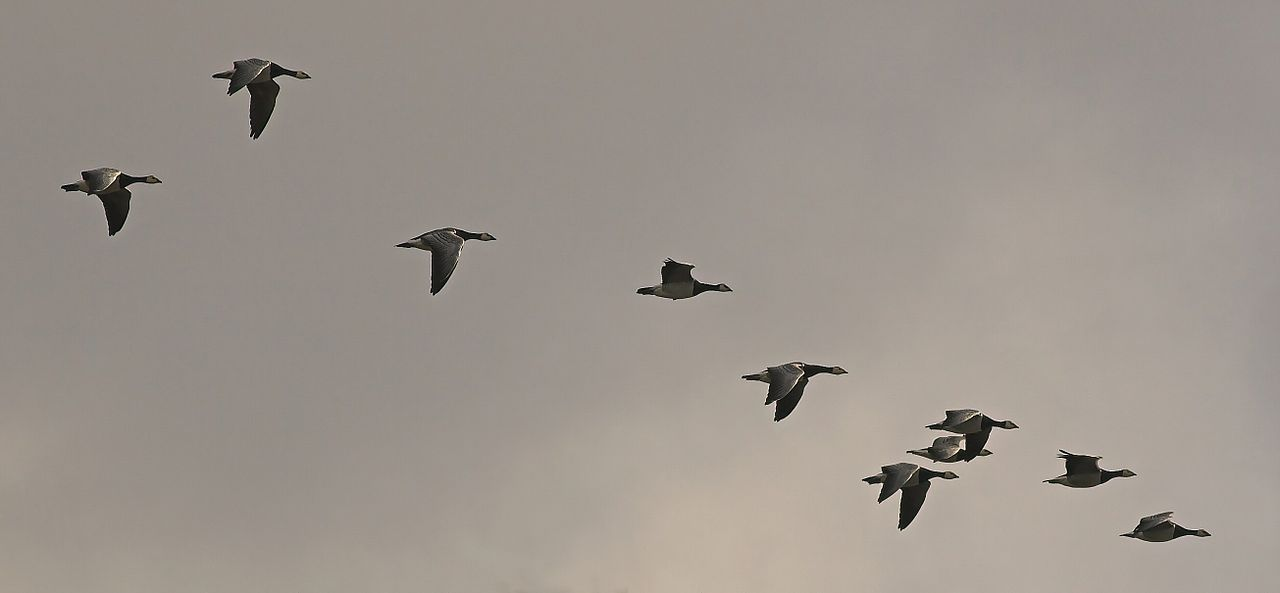
\includegraphics[width= 150pt]{Images/Oiseau.jpg}
     \caption{Image S}\label{Fig:Data2}
   \end{minipage}
\end{figure}

L'objectif est d'incruster toute ou partie de l'image S dans l'image T. En terme de manipulations, cela consiste à effectuer un copier/coller ou encore un clônage de la seconde image dans la première.
Le résultat que nous attendons pour une incrustation "réussie" est un résultat comme celui présenté ci-dessous : 
    
\begin{center}
\begin{figure}[!htb]
   \centering
     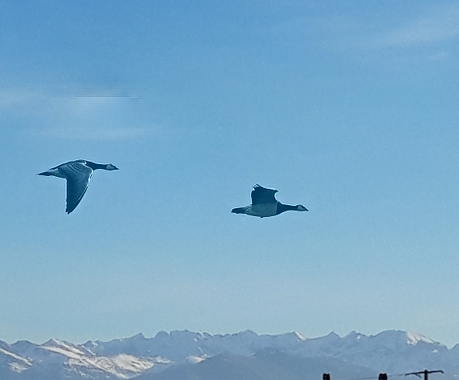
\includegraphics[width = 150pt]{Images/clonage_done.png}
     \caption{Image  finale attendue}
\end{figure}
\end{center}
Cette image est extraite d'une simulation effectuée sur \url{'demo.ipol.im/demo/163/'}. Nous comparerons les images obtenues à l'aide nos algorithmes avec celle-ci à la fin de ce rapport.\newline
\paragraph{Remarques}
Ce résultat est réussi parce qu'il semble naturel, les frontières entre l'image collée et l'arrière plan sont très peu visibles et ont été estompées, les oiseaux présents dans la première image n'ont pas été déformés et semblent faire parti de l'image. 
Mais comment obtenir un tel résultat ?
\newline
Reprenons nos deux images séparées, T et S et commençons par effectuer un simple copier/coller. Certains pixels de T sont donc écrasés par ceux de S. En effectuant cette manipulation voici l'image que nous devrions obtenir : 
\begin{center}
\begin{figure}[H]
     \centering
     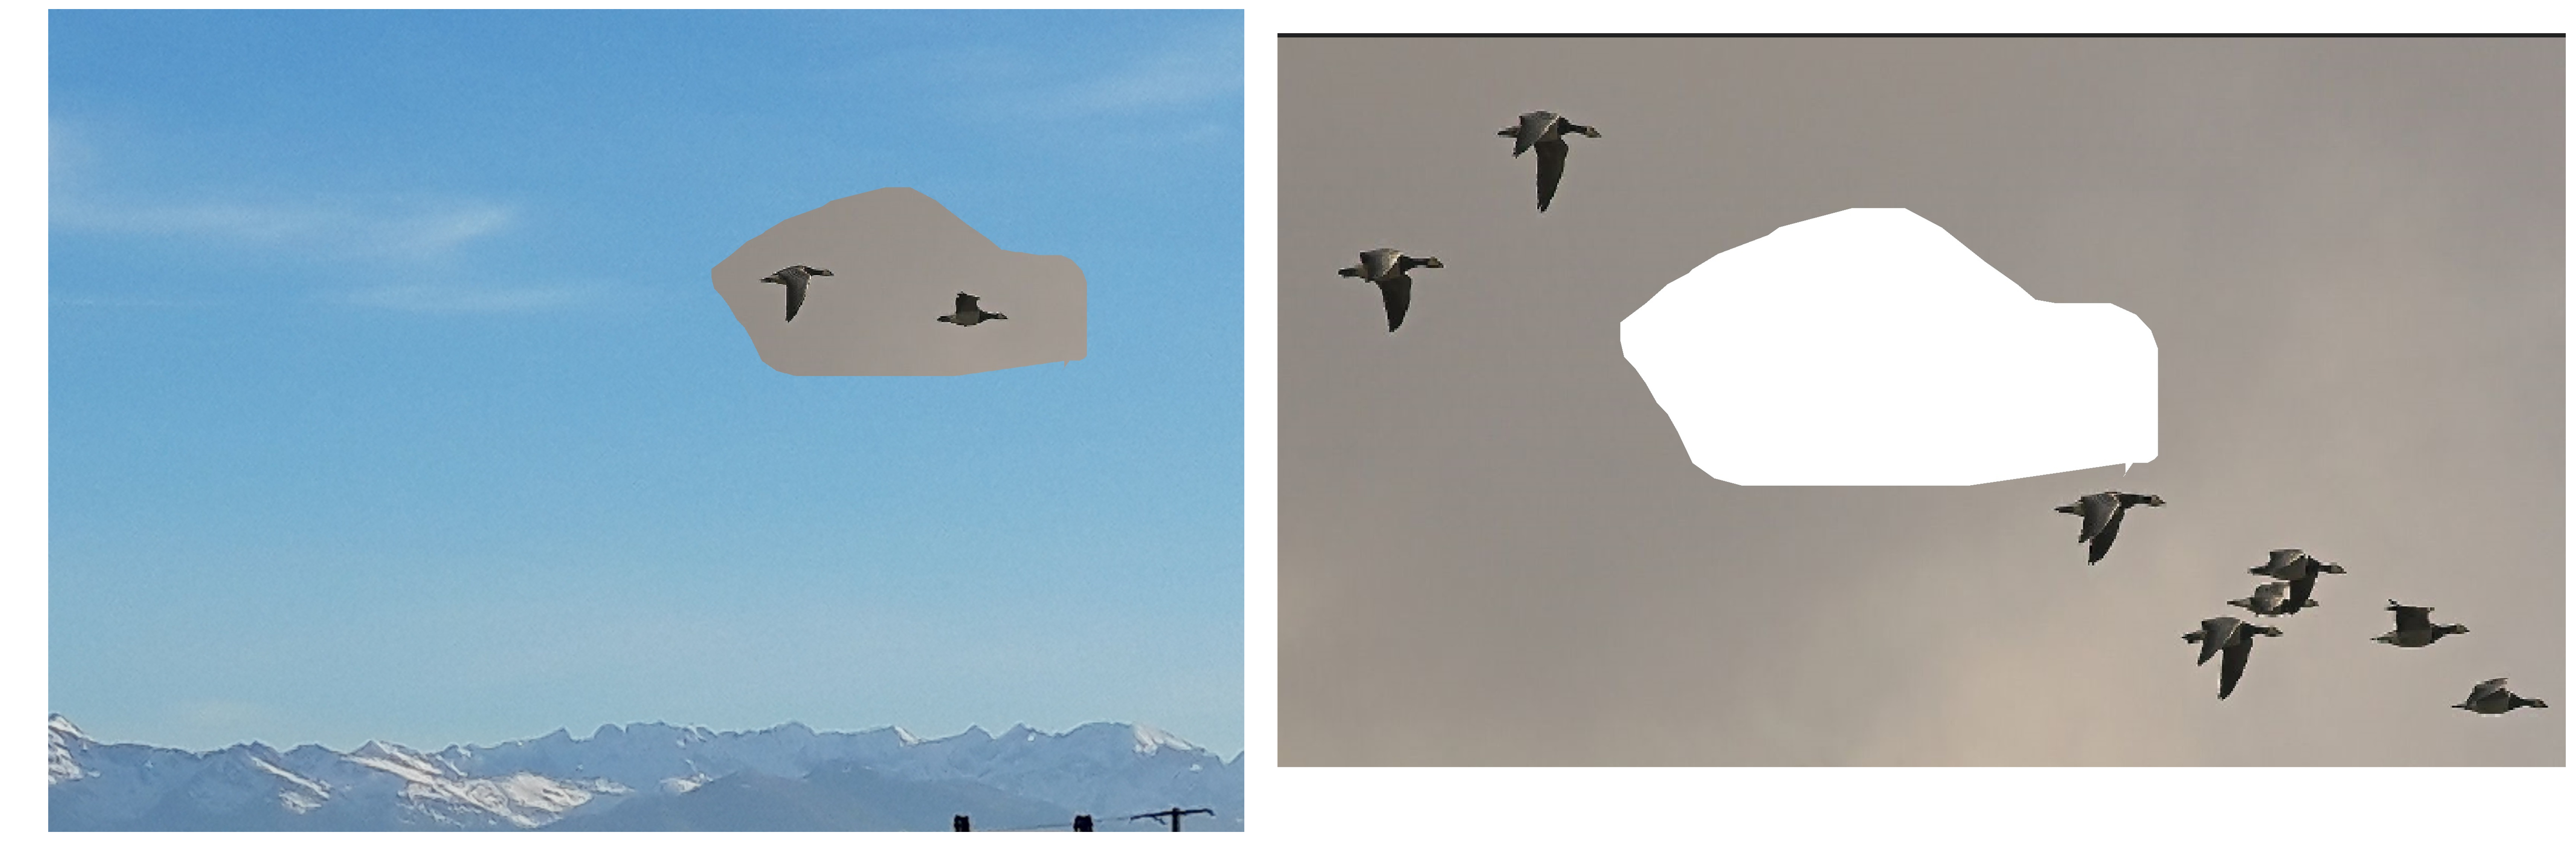
\includegraphics[width = 200pt]{Images/collage1.jpg}
     \caption{Simple copier/coller}
\end{figure}
\end{center}

Ce résultat n'est bien entendu pas convenable et bien loin de l'image finale attendue. Le découpage et le collage entre l'arrière-plan et l'image "objet" sont beaucoup trop visibles, les couleurs ne sont pas les mêmes et incohérentes. Nous souhaitons obtenir un résultat beaucoup plus naturel, comme écrit plus haut. Cette simple manipulation n'est donc pas suffisante pour effectuer le clônage cohérent  d'une image dans une autre. \newline

Il semble évident de vouloir modifier l'image finale obtenue ci-dessus afin qu'elle paraisse la plus naturelle possible.
Nous verrons tout au long de ce rapport, quels sont les changements à effectuer, et comment la résolution d'une équation aux dérivées partielles,l'équation de Poisson, nous permet d'obtenir un bien meilleur résultat. Nous implémenterons trois algorithmes permettant de résoudre le problème posé, et comparerons les résultats obtenus à l'aide de ceux-ci
%%%%%%%%%%%%%%%%%%%%%%%%%%%%%%%%%%%%%%%%%%%%%%%%%%%%%%%%%%
%           TRADUCTION SOUS FORMES MATHEMATIQUES         %
%%%%%%%%%%%%%%%%%%%%%%%%%%%%%%%%%%%%%%%%%%%%%%%%%%%%%%%%%%

\subsection{Problème mathématique associé}

Comme écrit plus haut nous souhaitons apporter des modifications au précédent collage afin qu'il corresponde au mieux à nos attentes. En réalité nous ne souhaitons pas modifier l'entièreté de l'image mais seulement un "sous-domaine" correspondant à l'endroit du collage. Pour ce faire, considérons I, la partie de l'image finale à modifier. Nous pouvons ainsi représenter le problème sous forme schématique. 
\begin{center}
    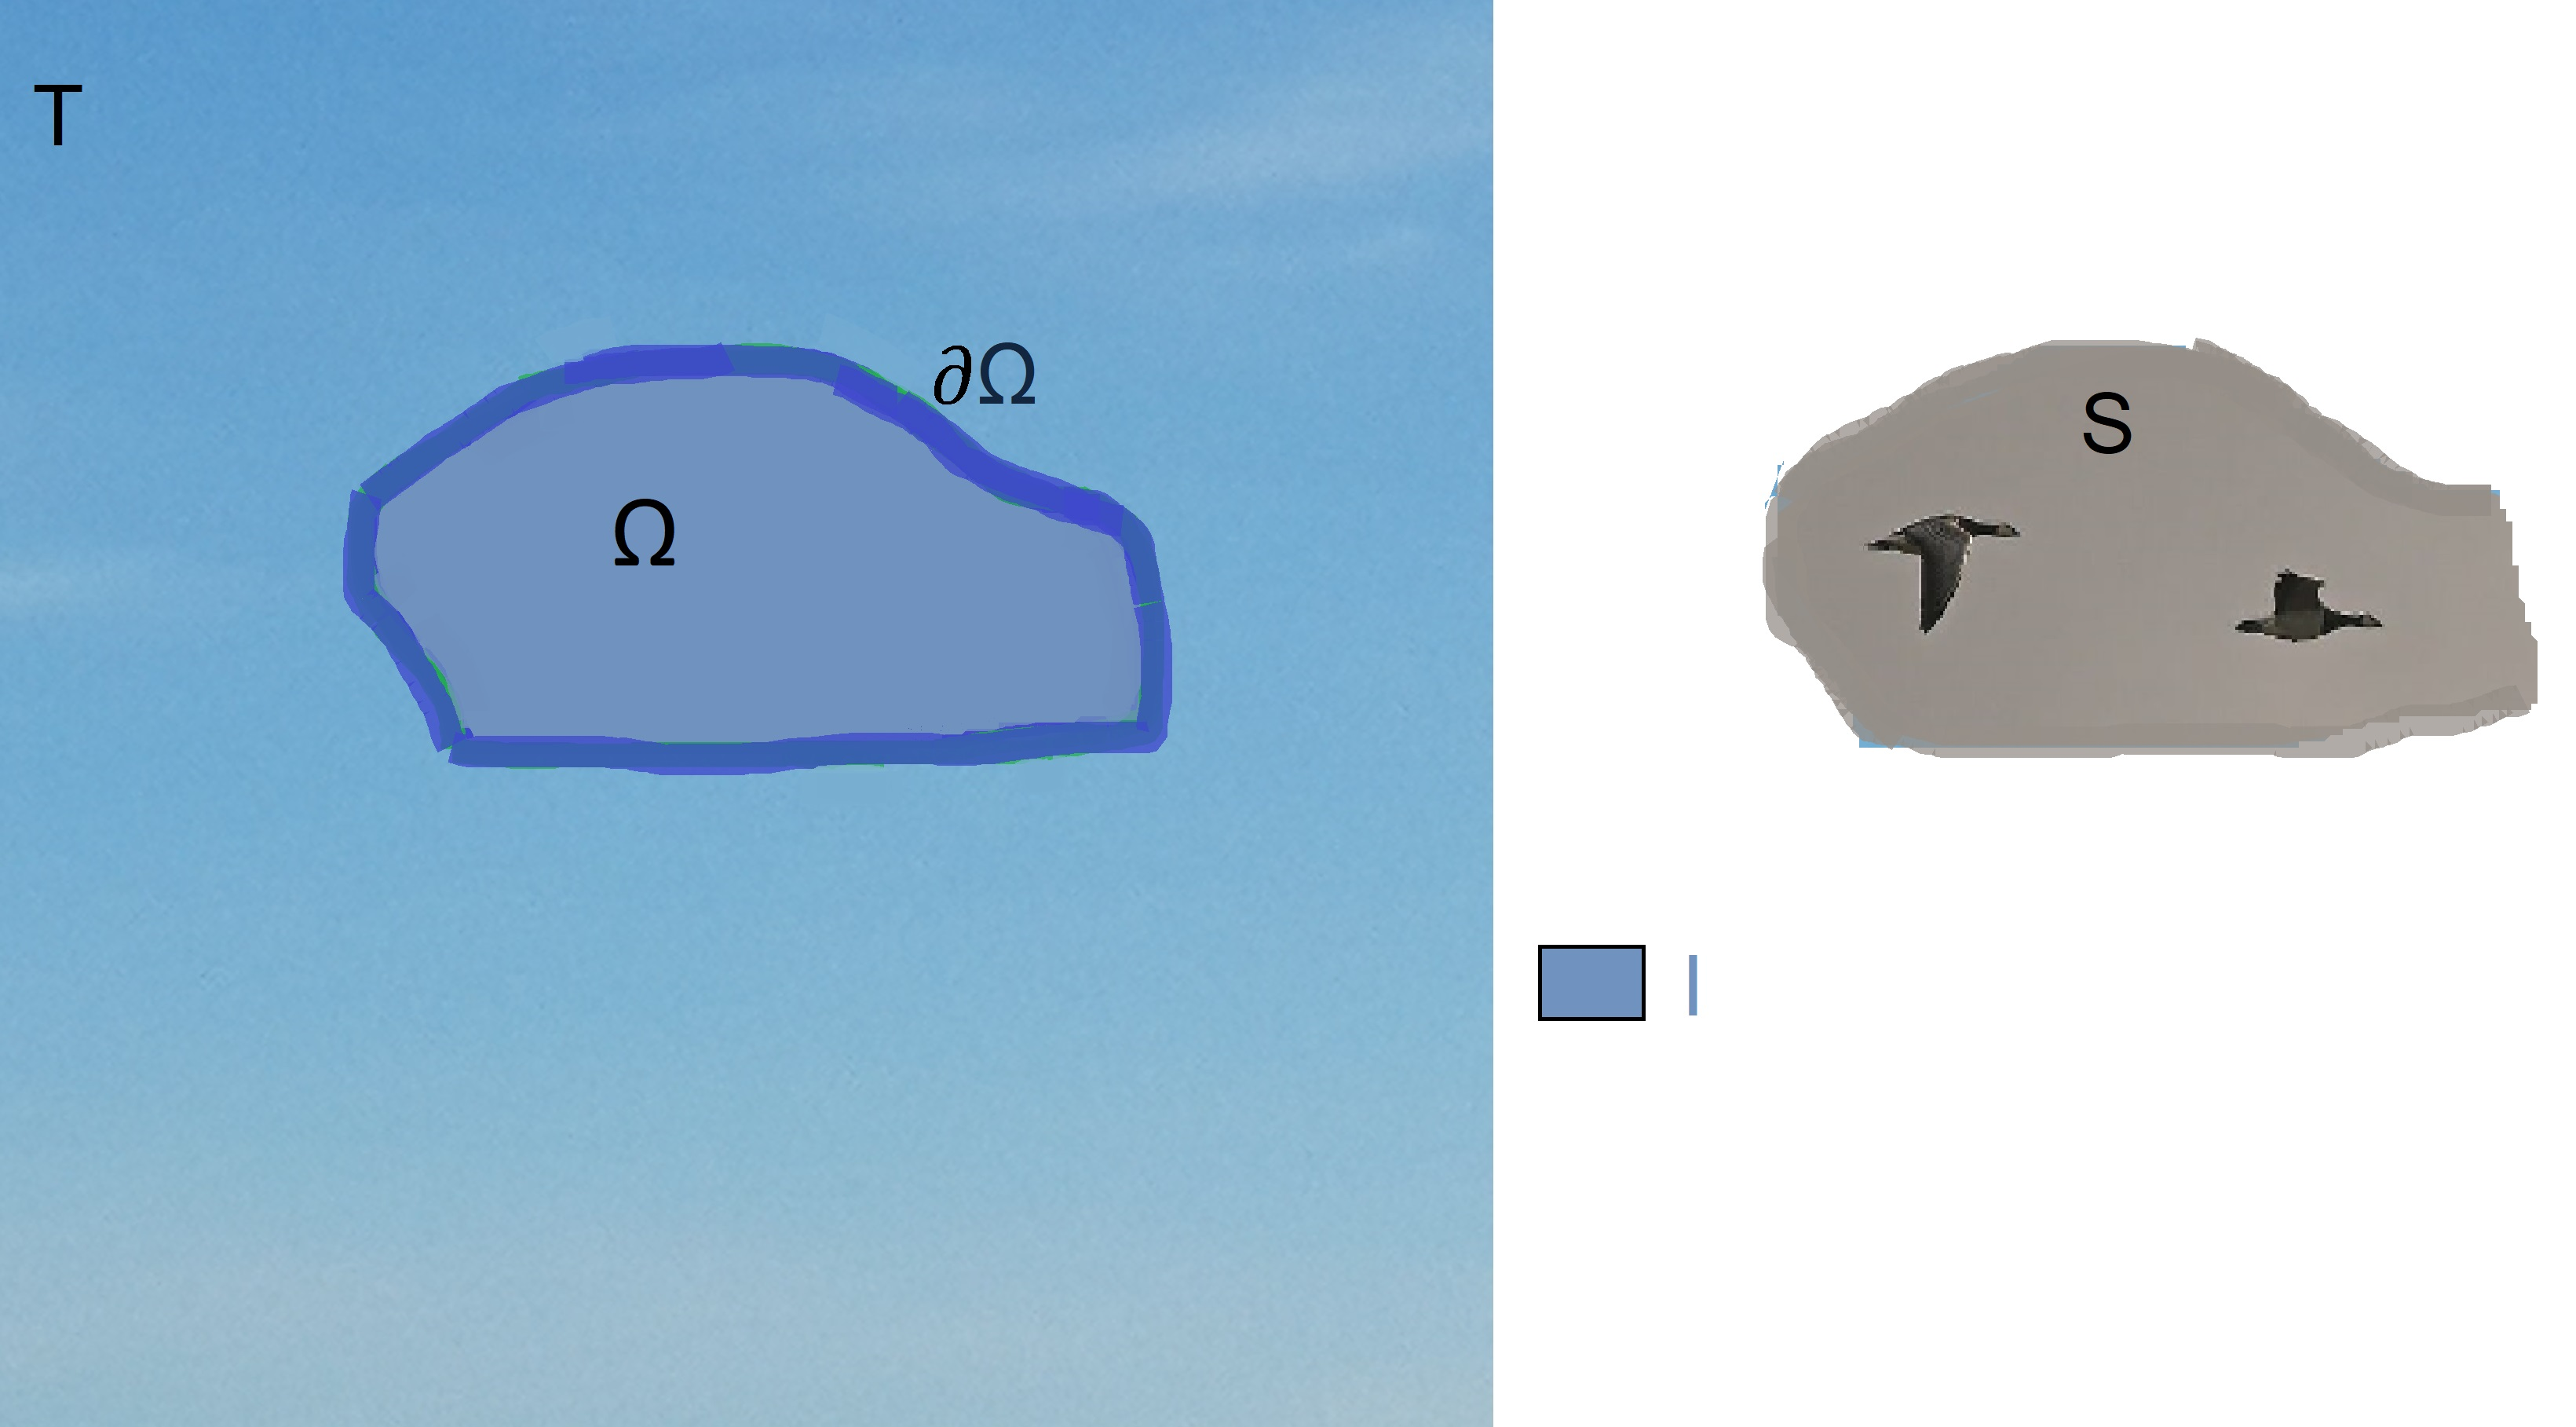
\includegraphics[width = 200pt]{Images/Schee.jpg}
\end{center}

Ici : 
\begin{itemize}
    \item T est l'image "Target", l'image destination, l'image sur laquelle s'effectuera le collage, l'arrière plan. 
    \item S est l'image "Source", l'image que nous souhaitons coller.
    \item $\Omega$ est le domaine dans lequel se trouvent nos inconnues.
    \item $\partial \Omega$ est la frontière de $\Omega$.
    \item I est notre inconnue, la partie de l'image que nous ne connaissons pas et que nous voulons remplir.
\end{itemize}

Nous souhaitons donc trouver une fonction I qui satisfasse un certain nombre de critères, afin de correspondre au résultat attendu.  
Cette fonction représente la partie modifiée de notre image. Mais quelles sont les conditions qu'elle doit remplir pour que le rendu soit le meilleur possible? Notre nouvelle image I doit-elle être plus proche de l'image collée S, ou de l'image d'arrière-plan T ? \newline
Pour répondre à cette question, reprenons le problème de départ. \newline

Pour que l'image obtenue s'incruste parfaitement,il faut que celle-ci dénature le moins possible les deux images sélectionnées au départ. En effet, nous devons garder les détails de l'image que nous voulons coller, S, ne pas modifier les variations qu'elle pourrait posséder comme par exemple, les contours ou les objets, lui appartenant.Nous devons donc pouvoir retrouver les informations présentes dans celle-ci. Par conséquent, il faut que les objets ou contours présents dans $I$ soient presque identiques à ceux de S.\\
Rappelons qu'en traitement d'image, les variations d'une image peuvent être obtenues en calculant son gradient. En effet, une variation peut-être représentée comme un changement "brutal" d'intensité entre deux pixels. Le gradient d'une image étant numériquement obtenu en effectuant la différence entre des pixels voisins : si celle-ci est élevée alors il y a une fort changement d'intensité entre eux, (par exemple un pixel noir et un autre blanc), et donc possiblement la présence d'un contour. Par conséquent, un fort changement d'intensité, implique un fort gradient. Au contraire, l'absence de variations entraîne un gradient presque nul. Son calcul permet entre autre de détecter les contours d'une image.\\
Nous souhaitons ici, que les contours et objets de l'image finale soient très proches de l'image à coller. Mathématiquement, nous voulons donc une fonction I dont le gradient est le plus proche possible, ou identique à celui de l'image collée, S. Nous cherchons donc :
\begin{center}
    $$ min \iint_\Omega || \nabla I_{x,y} - \nabla S_{x,y}||^2 dxdy$$
\end{center} 

Mais les "frontières" entre l'image collée et l'image d'arrière-plan T, ne doivent pas non plus être visibles, il faut donc que les pixels se situant sur cette partie là, i.e $\partial \Omega$, soient le plus proches possible de T .  Nous voulons donc, mathématiquement, chercher la fonction I qui vérifie: 
\begin{center}
    $I_{(x,y)} = T_{x,y} \ sur\ \partial \Omega$
\end{center}

Répondre au problème implique donc de résoudre un problème variationnel classique auquel des conditions sur le bord de Dirichlet sont ajoutées. 
Réécrivons le problème mathématique que nous cherchons à résoudre :  

\begin{center}
\begin{equation}
\left\{
\begin{aligned}
 min \iint_\Omega || \nabla I_{x,y} - \nabla S_{x,y}||^2 dxdy\\
 I_{(x,y)} = T_{x,y} \ sur\ \partial \Omega
\end{aligned}
\right.
\end{equation}
\end{center}


\subsection{Résolution et équivalence avec l'équation de poisson}
Pour résoudre cette équation, nous devons trouver le minimum de la fonction g suivante  : 
\begin{center}
\begin{equation}
\begin{aligned}
g(I) = \int_\Omega || \nabla I(x) - v(x)||^2 dx\\
\end{aligned}
\end{equation}
\end{center}
Si g admet un minimum alors, celui-ci annule son gradient. 
\subparagraph{Calcul de $\nabla g(I)$ }
À l'aide des formules de Taylor-Young à l'ordre 1 :\\
Soit f une fonction: $\mathbb{R}^n\rightarrow \mathbb{R}$ et $u \in \mathbb{R}^n$, tel que $||u||=1$ :
\begin{equation*}
\begin{aligned}
f(x_0+\epsilon u) = f(x_0) +\epsilon \left<\nabla f(x_0), u\right> + o(\epsilon)\\
\end{aligned}
\end{equation*}
En appliquant ces formules à notre cas :
\begin{equation*} 
\begin{aligned}
    g(I+\epsilon u) -g(I) =  \int_\Omega || \nabla (I+\epsilon u) - v||^2 - ||\nabla I -v ||^2 dx\\
\end{aligned}
\end{equation*}
En  développant : 
\begin{equation*} 
\left.
\begin{aligned}
    g(I+\epsilon u) -g(I) &=  \int_\Omega || \nabla I - v||^2+ ||\nabla \epsilon u||^2 +2(\nabla I - v)\times \epsilon \nabla u  - ||\nabla I -v ||^2 dx\\
  &=  \int_\Omega \epsilon ^2||\nabla u||^2 +2(\nabla I - v)\times \epsilon \nabla u dx\\
    & = 2\int_\Omega (\nabla I - v) \times (\nabla \epsilon u ) + O (\epsilon^2) \\ 
    & = 2\left<\nabla I - v, \nabla \epsilon u \right> + O (\epsilon^2) \\ 
      &  =   2\epsilon<\nabla I - v,  \nabla u> + O (\epsilon^2) \\ 
         &  = 2\left<\nabla I - v,  \nabla u \right> + O (\epsilon)\\ 
    & =  -2 <div(\nabla I - v), u > + O (\epsilon)\\
\end{aligned}
\right.
\end{equation*}
Par identification, le gradient de g vaut 
\begin{center}
		$\nabla g(I) = -2(\Delta I-div( v))$
\end{center} 
Le minimum de g annule son gradient donc on cherche I tel que : 
\begin{center}
		$0= (-\Delta I+div( v))$
\end{center}
Ici v = $\nabla S$ 
\begin{center}
		$\Delta I =div(\nabla S)$\\
		$\Delta I = \Delta S$
		
\end{center} 

Trouver le minimum de (2) revient donc à résoudre l'équation : 
\begin{center}
$\Delta I = \Delta S$
\end{center}
En remplaçant dans (1). On obtient le problème suivant : 
\begin{center}
    \begin{equation*}
        \left\{
        \begin{aligned}
         \Delta I = \Delta S  \ sur \  \Omega \\
          I = T \ sur \  \partial \Omega
        \end{aligned}
        \right.
    \end{equation*}
\end{center}
qui n'est autre que l'équation de Poisson, avec conditions aux bords de Dirichlet. 
Ainsi : résoudre le problème variationnel est équivalent à résoudre l'équation de poisson avec conditions aux bords de Dirichlet. Nous décrirons dans ce rapport 3 manières de résoudre cette équation. 

